\documentclass{beamer}

\usetheme{Berkeley}
\title{Implemention of an R Environments}
\author{Liam O'Suilleabhain\\ \bigskip YHAT}
\date{February 04, 2019}

\usepackage[utf8]{inputenc}
\usepackage{graphicx}
\usepackage{caption}
\usepackage{amsmath}
\usepackage{multicol}
\usepackage{hyperref} 
\usepackage{enumitem}
\usepackage{xcolor}
\usepackage{tikz}

\setbeamerfont{caption}{size=\tiny}

\usepackage{Sweave}
\begin{document}

\frame{\titlepage}



\setkeys{Gin}{width=0.6\textwidth}

\begin{frame}{Outline}
\begin{center}git clone https://github.com/losuilleabhain/AMORE.git \end{center}
\bigskip
\begin{itemize}
\item Introduction\\
\item Environment\\
\item Application\\
\item Implementation\\
\end{itemize}
\end{frame}

\section*{Introduction}

\begin{frame}{Motivation}
\begin{minipage}{0.6\textwidth}

\begin{center} Reproducibility necessitates a\\ \textbf{Standard Environment}\end{center} 
\bigskip

A Project has 3 sets of information
\bigskip
	
\begin{itemize}
\item[1] Resources
\item[2] Operations
\begin{small}
\begin{itemize}
\item \emph{A Functional Program \\ maps data to output}
\end{itemize}
\end{small}
\item[3] Results
\end{itemize}

\end{minipage}
\begin{minipage}{0.3\textwidth}
\begin{figure}
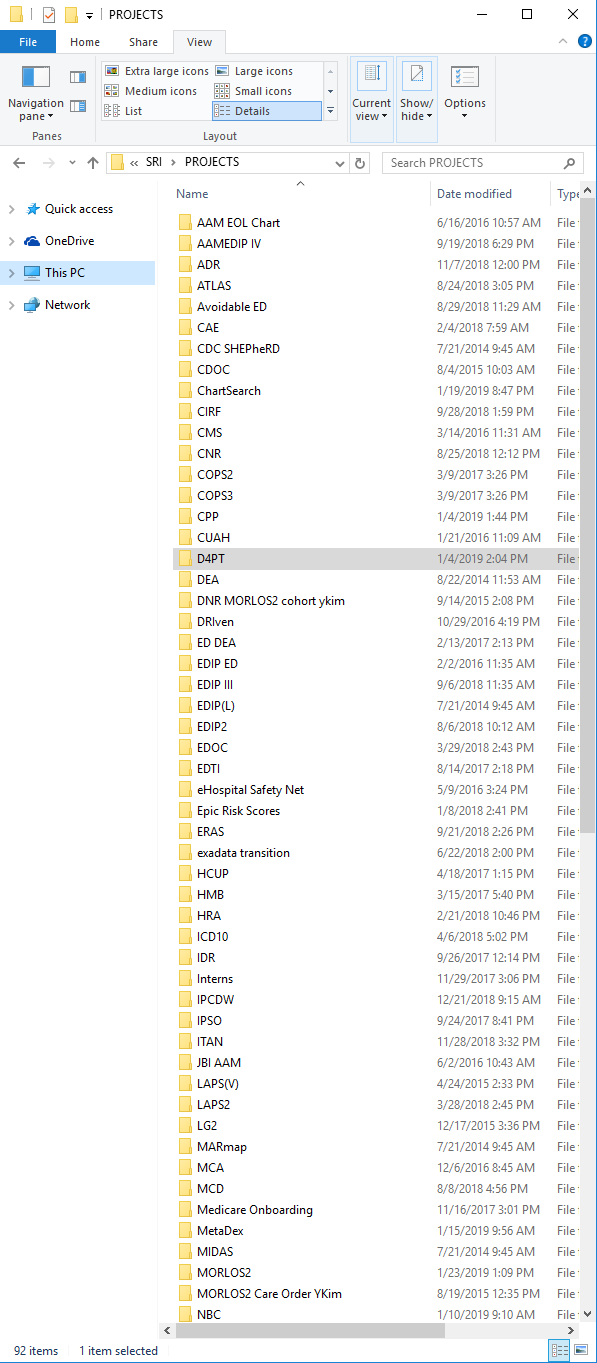
\includegraphics[width=0.9\textwidth]{./PROJECT_FOLDERS.PNG}
\caption*{ Many Shared Projects\\ Many Project Structures}
\end{figure}

\end{minipage}


\end{frame}


\section{Environment}

\begin{frame}{?Startup}
\begin{tiny}
Description:\\
\bigskip
In R, the startup mechanism is as follows.\\
\bigskip

Unless '--no-environ' was given on the command line, R searches
 for site and user files to process for setting environment
 variables.  The name of the site file is the one pointed to by the
  environment variable 'R\_ENVIRON'; if this is unset,
 {\color{red} 'R\_HOME/etc/Renviron.site' is used (if it exists, which it 
 does not in a `factory-fresh' installation)}.  The name of the user file
 can be specified by the 'R\_ENVIRON\_USER' environment variable; if
 this is unset, the files searched for are {\color{blue} '.Renviron' 
 in the	current or in the user's home directory (in that order)}.  See
 'Detailsr'’ for how the files are read.\\
\bigskip

Then R searches for the site-wide startup profile file of R code
 unless the command line option '--no-site-file' was given.  The
 path of this file is taken from the value of the `R\_PROFILE'
 environment variable (after tilde expansion).  If this variable is
 unset, {\color{blue} the default is 'R\_HOME/etc/Rprofile.site', 
 which is used if it exists (which it does not in a 'factory-fresh' 
 installation)}. This code is sourced into the 'base'package.  
 Users need to be careful not to unintentionally overwrite objects 
 in 'base', and it is normally advisable to use ‘local’ if code 
 needs to be executed: see the examples.\\
\bigskip

Then, unless '--no-init-file' was given, R searches for a user
 profile, a file of R code.  The path of this file can be specified
 by the 'R\_PROFILE\_USER' environment variable (and tilde expansion
 will be performed).  If this is unset, {\color{green} a file called 
 '.Rprofile' is searched for in the current directory or in the user's
 home directory (in that order)}.  The user profile file is sourced into
 the workspace.\\
\bigskip

\end{tiny}

\end{frame}

\begin{frame}{An R Environment}

\bigskip

\begin{minipage}{0.4\textwidth}

\begin{itemize}
\item 
\item[1.] R\_ENVIRON\\
\item[2.] R\_ENVIRON\_USER\\
\item[3.] R\_PROFILE\\
\item[4.] R\_PROFILE\_USER\\
\end{itemize}

\end{minipage}
\begin{minipage}{0.5\textwidth}

\begin{itemize}
\item 
\item {\color{red} R\_HOME/etc/Renviron.site\\}
\item {\color{blue} $\sim$/.Renviron}
\item {\color{blue} GROUP\_HOME/Rprofile.site\\}
\item {\color{green} $\sim$/.Rprofile\\}
\end{itemize}

\end{minipage}

\bigskip
\emph{Files in {\color{blue} blue} are available on github}

\end{frame}

\begin{frame}{One R Environment}

\begin{figure}[h!]
\begin{tikzpicture}      
\draw[blue, very thick] (0,5) rectangle (3,8) node[pos=.5] {
\includegraphics[width=0.25\textwidth]{R_logo.PNG}};
\end{tikzpicture}
\end{figure}
\begin{center}
\rule{4cm}{0.6pt}
\end{center}


\footnotesize
\begin{center}
\begin{tabular}{||c | c | c | c||}
\hline\hline
\textbf{Platform} & \textbf{Development} & \textbf{Notebooks} & \textbf{Datasets} \\
\hline
Machine & DOR Desktop & KPIT Server & DOR Server \\
\hline
Processor & 2.5GHz 4 Core &  2.3GHz 8 Core & 3.0GHz 32 Core \\ 
\hline
Memory & 16GB & 64GB & 256GB\\
\hline
Storage & Unlimited & 1TB & 1TB \\
\hline
Support & DOR IT & KPIT & DOR IT \\
\hline\hline
\end{tabular}
\end{center}

\end{frame}


\begin{frame}{Example: Set Environment Variable}
\bigskip
\begin{center}\textbf{ Example $\sim$/.Renviron on Unix\\} \end{center}
  R\_LIBS="$\sim$~/R/library"\\
\bigskip	
\begin{center}\textbf{ Example .Renviron on Windows\\} \end{center}
  R\_LIBS="C:/R/library"\\
\end{frame}

\begin{frame}{R\_ENVIRON - Global Environment (Optional)}

\begin{center}\$(R RHOME)/etc/Renviron.site\\ \end{center}
\begin{center}
\rule{4cm}{0.6pt}
\end{center}

\bigskip

\begin{center}Create a .Renviron file - $\sim$/.Renviron\\\end{center}
\textbf{Set R\_ENVIRON\_USER} \\

\end{frame}

\begin{frame}{R\_ENVIRON\_USER - User Environment}

\begin{center} $\sim$/.Renviron\\ \end{center}
\begin{center}
\rule{4cm}{0.6pt}
\end{center}

\begin{center}Create a group profile - GROUP\_HOME/Rprofile.site\\ \end{center}

\textbf{Set R\_PROFILE}

\begin{center}Create a shared library directory - GROUP\_HOME/R\_LIBS\\\end{center}

\textbf{Set R\_LIBS\_SITE}

\begin{center}Create a personal library directory - $\sim$/R\_LIBS\\\end{center}

\textbf{Set R\_LIBS\_USER}
\end{frame}

\begin{frame}{R\_PROFILE - Group Profile}

\begin{center} GROUP\_HOME/Rprofile.site\\ \end{center}
\begin{center}
\rule{4cm}{0.6pt}
\end{center}

\begin{center}Create .Rprofile - $\sim$/.Rprofile\\\end{center}
\textbf{Set R\_PROFILE\_USER\\}

\begin{center}
 Create Project .Rprofiles\\
\end{center}
\textbf{e.g. GROUP\_HOME/RPROFILE/.RPROFILE}
\begin{center} Create Function to source Project Environments \\\end{center}
\textbf{Define Renv}
\end{frame}

\begin{frame}{R\_PROFILE\_USER - User Profile {\color{green} (Freedom!)}}

\begin{center} $\sim$/.Rprofile\\ \end{center}
\begin{center}
\rule{4cm}{0.6pt}
\end{center}

\bigskip

\begin{center}
Create Development Directory e.g.\\ $\sim$/Development/ \\ 
\textbf{Set Development Directory}
\end{center}

\begin{center}
Create Password Vault \\ $\sim$/pwv.txt \\ 
\textbf{Load Passwords}\\
\end{center}

\end{frame}

\section*{Application}

\begin{frame}{A Project Profile}

\begin{center} GROUP\_HOME/RPROFILE/Rprofile.RPROFILE\\ \end{center}
\begin{center}
\rule{4cm}{0.6pt}
\end{center}

\begin{center}
Create Resource Directory\\
Create Code Directory \\ 
Create Analysis Directory\\
\end{center}

\textbf{Load Libraries\\}
\textbf{Set Project Options\\}
\textbf{Load Project Resources\\}
\textbf{Set Database Connections\\}

\end{frame}


\begin{frame}{Content Management}

\begin{minipage}{0.45\textwidth}
\begin{center}
\begin{figure}
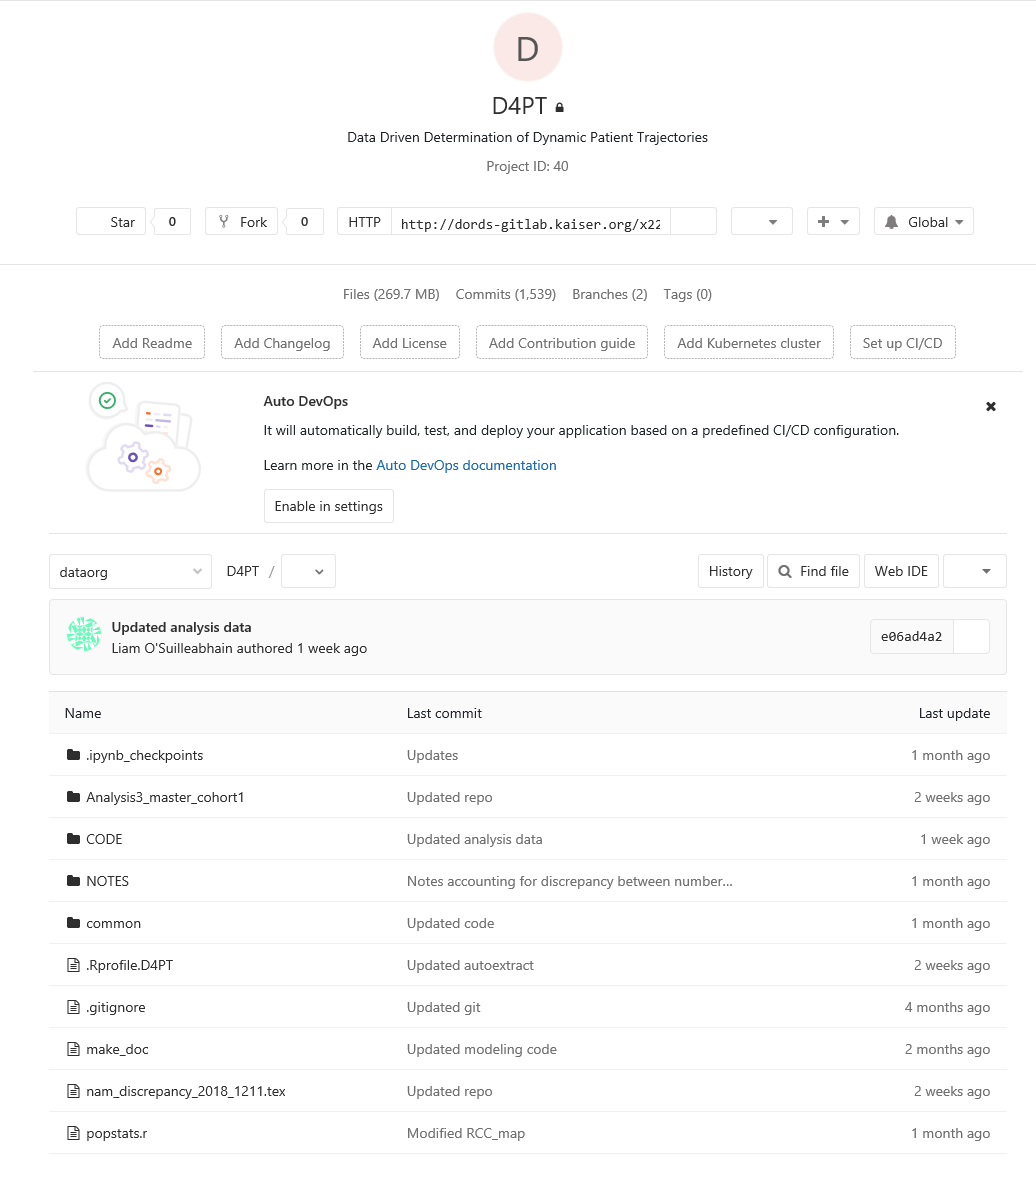
\includegraphics[width=0.9\textwidth]{./git.PNG}
\end{figure}
\end{center}
\end{minipage}
\begin{minipage}{0.45\textwidth}
\begin{center}
\begin{figure}
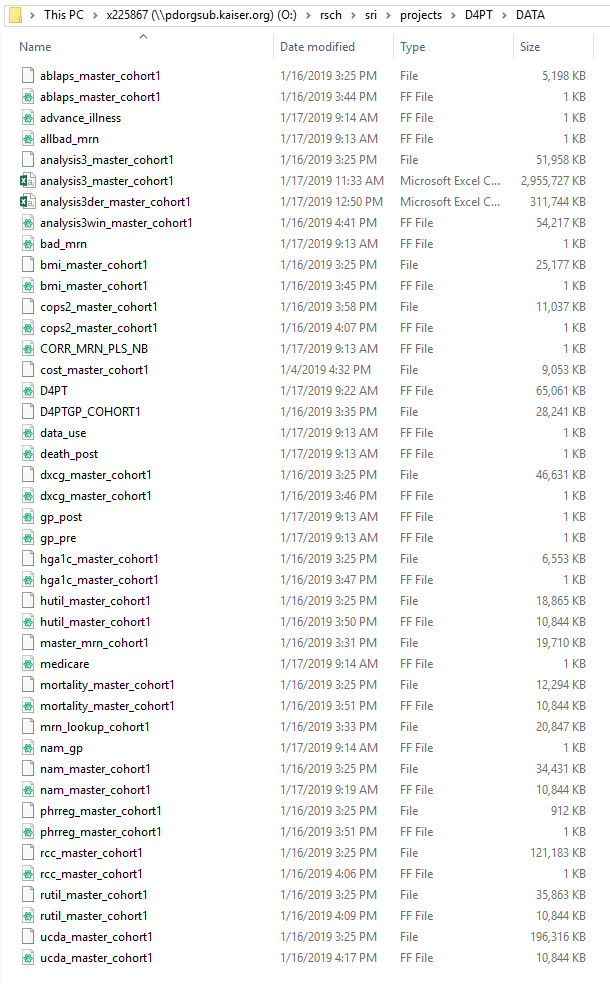
\includegraphics[width=0.9\textwidth]{./shared_data.PNG}
\end{figure}
\end{center}
\end{minipage}

\end{frame}

\section*{Implementation}

\begin{frame}{Project Workflow}

\textbf{Option 1:}
\begin{center}
Reference Files and Operations Relative to project path e.g.\\
source(``./CODE/analysis/models.r'')
\end{center}
\bigskip

\textbf{Option 2:}
\begin{center}
Separate git controlled code from the project e.g.\\
\begin{small}
ource(paste0(DATA,``analysis/models\_output''))
\end{small}
\end{center}
\bigskip

\end{frame}

\begin{frame}{Suggestions}

\emph{Only manage content that generates or contains analysis}

\begin{itemize}
\item \textbf{Management}
\begin{itemize}
\item Content
\item Structure
\end{itemize}
\end{itemize}
\bigskip

\emph{ Maintain same format for  Code and Analysis directories}
\begin{itemize}
\item \textbf{Maintenance}
\begin{itemize}
\item Operations - Code
\item Output - Analysis
\end{itemize}

\end{itemize}

\end{frame}

\begin{frame}{Future}

\textbf{Option 1 vs. Option 2}
\begin{itemize}
\item Option 1 is less verbose
\item Option 2 provides extra flexibility
\item Option 2 isolates code maintenance
\end{itemize}
\bigskip

\textbf{Develop Packages for Healthcare Analytics}
\bigskip

\textbf{Maintain git repositories with open-source code}

\end{frame}

\begin{frame}{Acknowledgements}

Thanks:

\bigskip

SRI for supporting this framework.\\
\bigskip

Chris Paciorek for ideas and advice.\\
\bigskip

Raj, Alejandro, Gina and Brian for helpful conversations.\\
 
\end{frame}
\end{document}


